\chapter{HISTORY OF MONEY}
\label{ch:historyofmoney}

Hoe zijn we hier gekomen? Hoe brengen we waarde over en hoe deden we dat in het verleden? Als je erover nadenkt, wat is dan een currency en wat is echt geld? In de loop van de geschiedenis hebben mensen waarde uitgewisseld van de ene persoon naar de andere door middel van handel, ruilhandel, het ruilen van goederen en diensten, maar vooral door gebruik te maken van iets wat we geld noemen. De crisis van 2008 heeft ons laten zien hoe kwetsbaar het huidige monetaire systeem is. Het huidige systeem is van nature gebrekkig, op schulden gebaseerd en niet duurzaam. Het komt een klein deel van de maatschappij ten goede, niet de massa. Als en wanneer gedistribueerde ledgertechnologie wordt toegepast voor het grotere goed, is het potentieel voor verstoring van de huidige orde enorm, met name in de financi\"ele dienstensector. Laten we, voordat we daarheen gaan, eerst de geschiedenis van het geld, fiat currency en het huidige monetaire systeem en beleid van vandaag bespreken.

\bigskip
\bigskip
\tcbset{colback=orange!3!white,fonttitle=\bfseries}
    \begin{tcolorbox}
    [enhanced,
    title=All Fiat Currencies become Worthless,
    frame style=
    {left color=orange!85!black,right color=yellow!95!black}]
    
      Door de gehele geschiedenis heeft geen enkele fiatvaluta ooit overleefd, en alle fiatvaluta's die ooit hebben bestaan, zijn naar een waarde van nul gegaan. \parencite{thebigreset}.
\end{tcolorbox}
\bigskip


\section{Eigenschappen van Geld}
Het bestaan van geld gaat duizenden jaren terug. Het geld dat we nu hebben en gebruiken is echter heel anders dan het geld dat we in het verleden hebben gehad. Laten we eens kijken naar enkele van de belangrijkste eigenschappen van 'sound money' [eerlijk geld] zoals gedefinieerd door internationaal gerenommeerde expert op het gebied van de geschiedenis van geld, Mike Maloney. In zijn boek Guide to Investing in Gold \& Silver: Protect your Financial Future, stelt Mike dat de volgende kenmerken 'sound money' defini\"eren:

\begin{enumerate}[label=(\alph*)]
    \setlength\itemsep{0em}
    \item Geld is een ruilmiddel
    \item Geld is een rekeneenheid
    \item Geld is duurzaam en bederft of corrodeert niet
    \item Geld is overdraagbaar
    \item Geld is deelbaar
    \item Geld is vervangbaar (elke eenheid is verwisselbaar)
    \item \textbf{Geld behoudt zijn waarde in loop van de tijd}
\end{enumerate}

\section{Sound Money}
Het eerste gezonde geld systeem dat in een bekende beschaving werd gebruikt, was gebaseerd op fysiek goud en zilver. Zuivere, geslagen munten zorgden ervoor dat regeringen, unilaterale organisaties en bankiers in toom werden gehouden omdat ze niet uit het niets nieuwe currencies konden cre\"eren. Een munt was ofwel sound money, ofwel gedekt door sound money. In het geval van beschavingen die echte gouden en zilveren munten gebruikten, ontstonden er pas problemen nadat regeringen hun muntstukken begonnen te devalueren. Dat betekent dat je je munt laat smelten en er een inferieur basismetaal aan toevoegt om het totale muntaanbod te vergroten. \parencite{goldsilver_ep1}.

\subsection{Store of value over time}
Het aanbod van goud is eindig, waardoor het in feite een schaarse bron is, zowel historisch als vandaag de dag. Het heeft en zal altijd nodig zijn voor mensen dat geld zijn waarde behoudt in de loop van de tijd. Het verzekeren van waardeopslag over een lange periode is een uitstekend voorbeeld van wat een grondstof als goud gezond geld maakt. Bovendien kan niemand uit het niets meer goud produceren of creëren, in tegenstelling tot het op fiat gebaseerde schuld-valutasysteem zoals we dat vandaag de dag kennen.


\begin{quotation}

      \textit{\say{500 voor Christus kon je voor \'e\'en troy ounce [31 gr] goud een Romeins senatorenkostuum kopen, in de 19e eeuw kon je voor \'e\'en troy ounce goud een Brooks Brothers kostuum kopen en vandaag de dag is een nieuw Italiaans kostuum \'e\'en ounce goud waard.}}
      \begin{flushright}
        \small{--- \textbf{R.W. Jastram}}
      \end{flushright}
    
\end{quotation}




\section{Fake Money, Fake System}
Helaas onderbouwen landen vandaag de dag niet meer hun currencies  met grondstoffen zoals goud. Laten we bijvoorbeeld eens kijken naar de U.S. dollar (US\$), die we vandaag de dag kennen als geld, maar in feite gewoon currencies zijn.\medskip

De inherente gebreken van het monetaire systeem hebben ons door verschillende bedrijfs- en financi\"ele cycli geleid die hebben geresulteerd in de zogenaamde \say{booms} en \say{busts} in activaprijzen. Sinds de \$USD van de goudstandaard ging in 1971, zijn er geen beperkingen meer op het gebied van de geldhoeveelheid, omdat het systeem niet meer wordt ondersteund door sound money. Uiteindelijk leidt dit tot een situatie waarin financiële producten, die geen waarde toevoegen aan de economie, exponentieel worden gecre\"eerd.


in het proces hebben financi\"ele instellingen, tussenpersonen en banken, die de makers zijn van die schuldproducten, veel winst gemaakt en tegelijkertijd een enorme hoeveelheid schuld gecre\"eerd. Bovendien neemt de verhouding van geld dat naar producten of diensten gaat die waarde toevoegen aan de economie en de maatschappij af naarmate de financi\"ele producten toenemen. De financi\"ele sector is booming, omdat er geen beperkingen zijn met betrekking tot de geldhoeveelheid, waardoor ze uit het niets krediet kunnen toveren in vormen van schuld en leningen en geld kunnen verdienen aan de rente. Schuld is het product van de financi\"ele industrie, en hoe meer schuld in de maatschappij wordt gecre\"eerd door banken, hoe meer macht naar de banken sector vloeit.

\medskip


\tcbset{colback=orange!3!white,fonttitle=\bfseries}
    \begin{tcolorbox}
    [enhanced,
    title=Nixon shock - off the gold standard,
    frame style=
    {left color=orange!85!black,right color=yellow!95!black}]
    
           Sinds de Verenigde Staten de converteerbaarheid van de Amerikaanse dollar US\$ in goud met de "Nixon Shock" in de jaren 70 hebben de nationale valuta's vrij zwevende koersen. Het monetaire beleid van de centrale banken heeft deze koersen voornamelijk gedicteerd. In 1971 nam de Nixon regering de internationale dollar van de goudstandaard af en vanaf dat moment keerde de VS terug naar een systeem dat alleen nog maar afhankelijk was van fiat valuta's, waarbij de US\$ alleen nog maar ondersteund werd door schulden en beloftes. 
      
\end{tcolorbox}
\medskip

Deze beslissing heeft vandaag de dag nog steeds invloed op de wereld, omdat de Amerikaanse dollar de wereldwijde reservevaluta was - en nog steeds is. Sindsdien hebben banken en financi\"ele tussenpersonen, maar ook currency makers zoals de Amerikaanse Federal Reserve, de Bank of Japan, de Europese Centrale Bank (ECB) en de Bank of China veel controle en invloed op de geldhoeveelheid. 

\section{Fiat currency}       
Fiat currency is een valuta die bestaat bij het dictaat of door fiat van een regering en/of bank (fiat is een Latijns woord voor een valuta die opgelegd in omloop is). Fiat currencies zijn inderdaad overvloedig en ruim beschikbaar binnen de jurisdicties waar ze worden geaccepteerd. Modern papiergeld en munten zijn, samen met hun digitale tegenhanger, enigzins duurzaam; fiat currency kan echter niet langer aanspraak maken op enige intrinsieke waarde. De waarde ervan wordt ervaren op basis van geloof en vertrouwen, en dat vertrouwen komt voort uit de steun van de respectieve overheden en een nationaal of internationaal vertrouwen in de stabiliteit van de munt.

Geen enkele regering of bank heeft ooit haar monetaire beleid kunnen disciplineren. De geschiedenis heeft aangetoond dat de invoering van een fiat currency model het voor elke regering gemakkelijker maakt om een van de volgende dingen te doen. Herinner dat er dus geen limiet aan de hoeveelheid van fiat currency zit omdat de munt zelf geen intrinsieke waarde heeft en niet wordt gedekt door gezond geld zoals goud);

\begin{enumerate}[label=(\alph*)]
    \setlength\itemsep{0em}
    \item Vergroot de geldhoeveelheid door te lenen
    \item Verhoog de geldvoorraad door eenvoudigweg te printen en het de maatschappij in te vloeien
    \item Verhoog van publieke uitgaven door de overheid
    \item Leg zware regelgeving op aan kleine bedrijven en voer een monetair beleid uit om de controle ervan verder uit te breiden
\end{enumerate}

\noindent Door de geschiedenis heen heeft geen enkele fiat currency ooit overleefd, en alle fiat currencies die ooit hebben bestaan zijn naar een waarde van nul gegaan. \parencite{thebigreset}. Als je dit vergelijkt met goud, is dit heel anders. Het maakt niet uit of een gouden munt \$120 of \$15.000 dollar waard is. De waarde ligt in wat voor echte goederen of diensten je ermee kunt kopen, niet de absolute waarde uitgedrukt in \'e\'en of andere (nationale) fiatvaluta. 

\begin{quotation}

      \textit{\say{Papier geld keert uiteindelijk terug naar zijn intrinsieke waarde - nul.}}
      \begin{flushright}
        \small{--- \textbf{Voltaire}}
      \end{flushright}
    
\end{quotation}

\section{Koopkracht}
Het vergelijken van goud met elke fiat currency is als het vergelijken van appels met sinaasappels. Als we het hebben over fiat currency hebben we het over papieren fiat currency (contant geld) en digitale fiat currency (op je bankrekening).  Fiat-valuta voldoet aan twee voorwaarden van 'echt geld': het is een rekeneenheid en een ruilmiddel. Fiat-currency is echter geen waardeopslag over een lange periode.  Elke fiat currency die door een overheid wordt gecre\"eerd, heeft de neiging om in de loop van de tijd om verschillende redenen aan waarde in te boeten. \'E\'en daarvan is inflatie. Inflatie is het resultaat van te veel geld dat achter te weinig goederen aanzit, waardoor je fiatcurrency in waarde daalt naarmate de geldhoeveelheid groter wordt. 

Bijvoorbeeld, een inflatie van meer dan 2\% per jaar, wat tegenwoordig gebruikelijk is in de westerse wereld, vermindert je spaargeld in termen van wat je ermee kunt kopen (koopkracht) in 25 jaar tijd met de helft. Zonder rekening te houden met de consumenteninflatie voor producten; dezelfde prijs voor kleinere hoeveelheden van hetzelfde product. Inflatie vindt plaats over een zeer lange tijd, en veel mensen realiseren zich niet dat hun munt langzaam maar zeker waardeloos wordt - als een tijdbom die op het punt staat te exploderen. Als de op fiat gebaseerde economie uiteindelijk instort na zoveel rondes van kwantitatieve versoepeling [quantitative easing] en hyperinflatie, zijn de uitkomsten meestal catastrofaal. \parencite{weimarhyperinflation}. \medskip

\medskip

    \tcbset{colback=orange!3!white,fonttitle=\bfseries}
    \begin{tcolorbox}
    [enhanced,
    title=Banking system,
    frame style=
    {left color=orange!85!black,right color=yellow!95!black}]

         \itshape{The rules of money and banking have changed every 20 or 30 years for the past three centuries, in an ongoing trial-and-error experiment in evolving a financial system, and a constant battle over whose interests it will serve. To present that timeline in full will take another article, but in a nutshell, we have gone from precious metal coins to government-issued paper scrip, to privately-issued banknotes, to chequebook money, to gold-backed Federal Reserve Notes, to unbacked Federal Reserve Notes, to the \say{near money} created by the shadow banking system. Money has evolved from being \say{stored} in the form of a physical commodity to paper representations of value, to computer bits storing information about credits and debits.}
        
        \tcblower
        
        \textbf{The rules have been changed before and can be changed again.} Depressions, credit crises and financial collapse are not acts of God but induced by mechanical flaws or corruption in the financial system. Credit may stop flowing, but the workers, materials and markets are still there. The system needs a reboot. Hopefully, the next program that gets run will last more than 20 or 30 years. Ideally, we might mimic the ancient Mesopotamians, the oldest and most long-lasting civilisation in history, and devise an economic system that lasts for millennia.\cite{EllenBrown}

\end{tcolorbox}

\medskip

\noindent Toen de wereld van de goudstandaard afging, waren centrale banken en regeringen aan niemand verantwoording schuldig of werden ze gedwongen de geldhoeveelheid te beperken (omdat die niet meer gekoppeld was aan iets met echte waarde). Het niet hebben van de vereiste om gedrukt geld te ondersteunen met een fysiek goed heeft geleid tot een explosie van schulden in de vorm van financi\"ele producten. De financiële sector verhandelt nu triljoenen in financiële producten, de effecten daarvan zijn zichtbaar in veel economische indicatoren.\medskip


\section{Bedenkelijk Monetair Beleid}
Verschillende andere factoren en partijen vernietigen de koopkracht van de fiatvaluta. Als een regering eenmaal een fiatvaluta heeft ingevoerd, kan ze meestal de verleiding niet weerstaan om het valutabestand uit te breiden door middel van uitgaven voor tekorten (verhoging van het plafond van de overheidsschuld). Commerciële banken creëren geld uit het niets door fractioneel reservebankieren. Centrale banken creëren geld door leningen te verstrekken aan overheden en commerciële banken. Bovendien voeren sinds 2008 bijna alle centrale banken ter wereld, zoals de Europese Centrale Bank, de Federal Reserve, de Bank of England en de People's Bank of China, het beleid uit van wat zij noemen Quantitative Easing (QE). QE is een expansief monetair beleid waarbij een centrale bank vooraf bepaalde bedragen aan staatsobligaties of andere financiële activa koopt om de economie te stimuleren en de liquiditeit te vergroten. Het is een onconventionele vorm van monetair beleid en wordt meestal gebruikt wanneer de inflatie zeer laag of negatief is en het standaard expansieve monetaire beleid ineffectief is geworden.

This policy is nothing more than a process where the authoritative body injects an insane quantity of currency into the economy at near 0\% interest rates to serve as a stimulus for the economy. Also referred to as "credit expansion but ultimately, it's just more debt. Refer to \cref{fig:fedgraph_debt_EU,fig:fedgraph_debt_US,fig:fedgraph_debt_JPN} for an impression of ever-increasing debt levels (as a \% of GDP) for the US, EU and Japan. There are now many countries around the world where this policy is applied.


    \begin{figure}
        \centering
        \caption{Central Government debt, total \% of GDP for the Euro Area}
        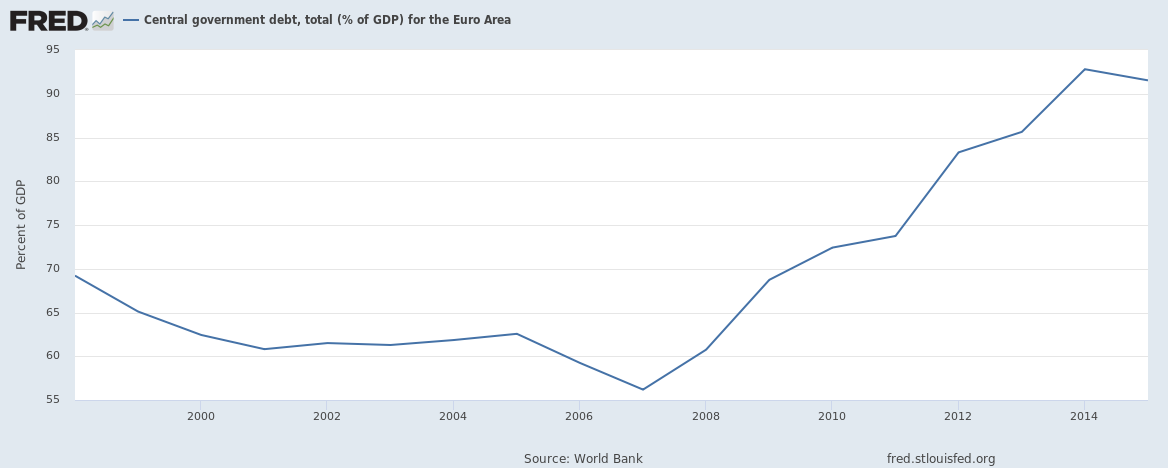
\includegraphics[width=\textwidth]{img/ch-history/fredgraph_debt_EU.png}
       
        \label{fig:fedgraph_debt_EU}
        \source{Federal Reserve Bank of St. Louis, Economic Research \parencite{FRED}.}
    \end{figure}
    
    \begin{figure}
        \centering
        \caption{Federal Government total public debt as a \% of GDP for the US}
        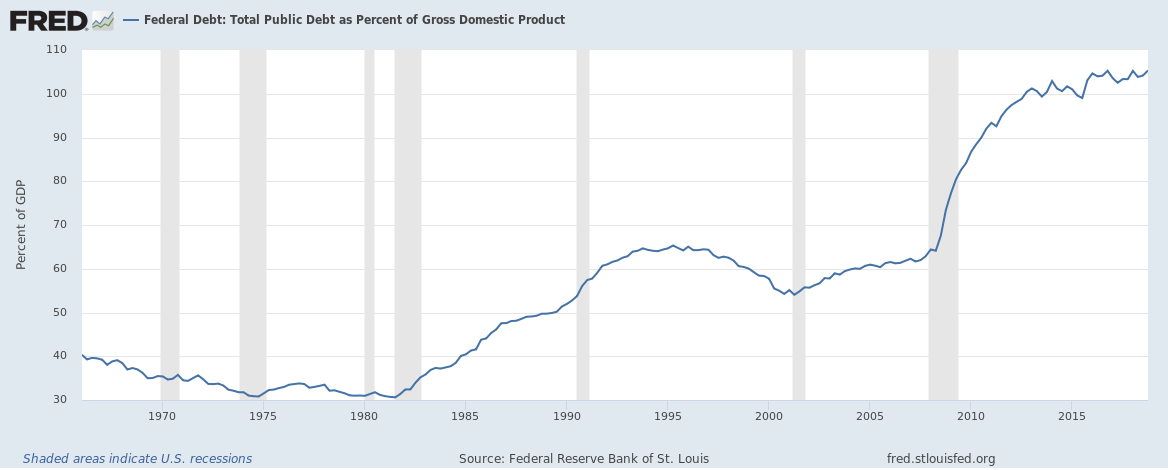
\includegraphics[width=\textwidth]{img/ch-history/fredgraph_debt_US.png}
       
        \label{fig:fedgraph_debt_US}
        \source{Federal Reserve Bank of St. Louis, Economic Research \parencite{FRED}.}
    \end{figure}
    
    \begin{figure}
        \centering
        \caption{Central Government debt, total \% of GDP for Japan}
        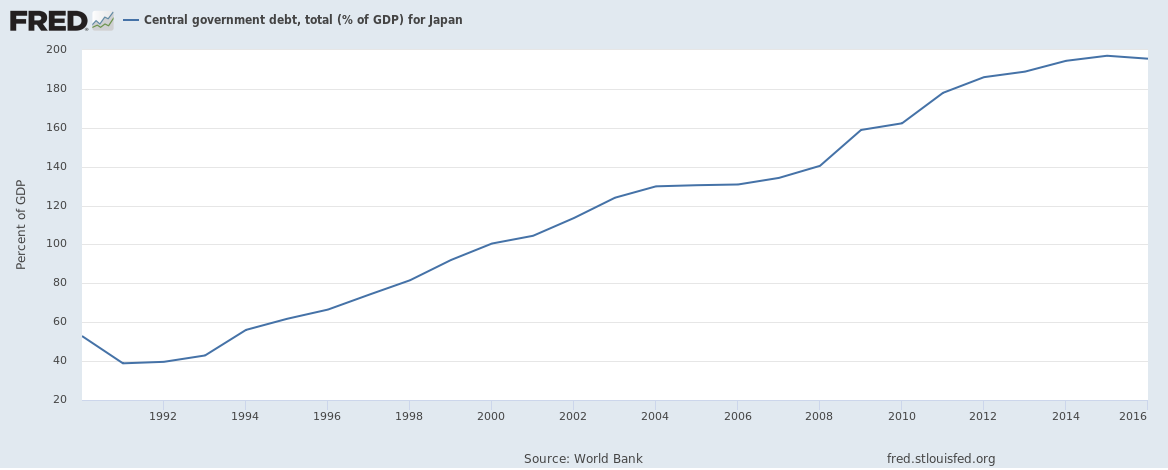
\includegraphics[width=\textwidth]{img/ch-history/fredgraph_debt_JPN.png}
       
        \label{fig:fedgraph_debt_JPN}
        \source{Federal Reserve Bank of St. Louis, Economic Research \parencite{FRED}.}
    \end{figure}

\section{Post financial crisis 2008}
        
The result was an even more gigantic debt bubble that heralded the financial crisis of '08. Inevitably, when interest rates are going to rise again, the lion's share of all debtors will have immense problems to pay off their debt plus added interest.\medskip 



\begin{quotation}

      \textit{\say{In 2000 we had the dot-com bubble. In 2008 we had the housing bubble. In 2019 we have the \emph{everything} bubble}}
      \begin{flushright}
        \small{--- \textbf{Mauldin Economics}}
      \end{flushright}
    
\end{quotation}


In the previous financial crashes, central banks had an opportunity to stimulate the economy by lowering interest rates, which made capital less expensive so people could lend more. Ten years after the last crash, interest rates are still near zero. Having interest close to zero provides very little to no room to lower interest rates (again) and 'save' us from yet another depression. In 2008, they just delayed the inevitable, but in the future, we will have to deal with the consequences.\medskip

On top of this, by creating enormous amounts of fiat currency, the money supply expands, and more currency is chasing the same amount of goods and services, which results in high inflation rates. High inflation rates result in higher prices for products and services. Moreover, eventually, when all fiat (digital) currency is circulating in the economy, it could result in a global fiat currency crisis through hyperinflation. \Cref{tab:inflationratescountries} shows countries with high inflation rates. Highest inflation rate by country in 2019. The highest inflation rate in 2019 was reported in Venezuela, followed by Zimbabwe, South Sudan, Sudan, Argentina, Liberia, Iran and Ethiopia, Haiti and Angola. Note that Venezuela has suffered from severe hyperinflation. Such an event has the potential to obliterate the saving accounts of entire generations, and all of our currency suddenly becomes worthless paper. 

\begin{table}
\centering
\caption{Inflation rates $>$ 20\%}
\begin{tabular}{@{}lllll@{}}
\toprule
\textbf{Country} & \multicolumn{3}{l}{\textbf{Inflation rates {[}\%{]}}} \\ 
\textbf{}        & Q4 ''18          & Q1 ''19          & Q2 ''19    & Q4 ''19     \\ \midrule
Venezuela        & 1698488          &                  & 282973     & 39114    \\
Argentina        & 47.1             &                  & 57.3       & 52.9    \\
Sudan            &                  & 43.5             & 44.6       & 57.7    \\
South Sudan      & 33.5             &                  & 56.1       & 69    \\
Zimbabwe         & 42.1             &                  & 97.9       & 521   \\
Iran             & 39.9             &                  & 52.2       & 27.8     \\
Liberia          & 26.6             &                  & 23.3       & 30.9     \\
Turkey           &                  & 20.4             & 18.7       & 11.8           \\ \bottomrule
\end{tabular}
\source{Trading Economics, 24-01-2020. \emph{Inflation Rate - World.} \parencite{tradingeconomics}}
\label{tab:inflationratescountries}
\end{table}


\noindent In short, the history of fiat currencies is a history of volatility. The average lifespan of a fiat currency is only twenty-seven (27) years. Even if a currency survives any longer, invariably it will experience increasing inflation. Inflation steadily erodes the purchasing ability of fiat money over time. The world's oldest fiat currency, the British pound (\pounds), is an excellent example; it has lost ninety-nine and a half per cent (99.5\%) of its value since inception. Historically gold is more resilient, and holds its value better than any fiat currency and is particularly strong in times of economic instability.

\section{Legacy financial infrastructures}

At present, we mostly rely on middlemen or intermediaries like banks, commerce platforms or governments to establish the element that allows our economy to function in a digitized space: trust. These third parties perform the transactions in such a way to enable authentication, record-keeping or payment clearance to ensure that both parties in a transaction oblige to some pre-specified terms and conditions, and thus allowing the buyer and seller to remain confident that the transaction will execute securely and effectively.
While these intermediaries are crucial to our digital economy, there are some significant issues.

\begin{itemize}
    \setlength\itemsep{0em}

    \item They use centralized databases which face high risks of being hacked
    \item They exclude billions of people, who lack access to resources and capital, from the global economy
    \item They charge transaction fees in the form of hefty commissions, not to mention the major timing inefficiencies
    \item They undermine the privacy of the users when they track and use our data as a function of their marketing efforts and business model
    \item They have appropriated the largest of the digital age asymmetrically, as we have wealth creation but growing economic and social inequality
\end{itemize}

\begin{quote}
    \textbf{\emph{Follow the Rabbit: Enter blockchain}}
\end{quote}


